\documentclass[10pt,a4paper]{article}
\usepackage[margin=20mm]{geometry}\usepackage[T1]{fontenc}\usepackage{lmodern,microtype,booktabs,graphicx,xcolor,hyperref,tcolorbox,parskip}
\setlength{\emergencystretch}{3em}
\definecolor{ink}{HTML}{172B4D}\definecolor{teal}{HTML}{167C80}\definecolor{mist}{HTML}{F1F6F8}
\hypersetup{colorlinks=true,linkcolor=teal,urlcolor=teal}
\title{\vspace{-2em}\color{ink}\bfseries IDM-Viz label audits on NOAA observations\\[-.2em]\large A retrospective known-probability sampling replay}
\author{Phase 3 supplementary experiment}\date{17 November 2026}
\begin{document}\maketitle\vspace{-1em}
\begin{tcolorbox}[colback=mist,colframe=teal,boxrule=0pt,leftrule=2mm]\textbf{Scope boundary.} This replays randomized label selection on one previously observed NOAA station chronology. It is not prospective label operations, independent domain replication, or a weather forecast.
\end{tcolorbox}
\section*{Design}
The existing frozen logistic model was refit from the same historical partitions and its batch accuracies were required to match the locked NOAA evaluator exactly. The monitoring sequence contributes 21 complete batches of 500 rows (10,500 total); the final 426 rows are excluded, matching the original evaluation. For each batch, policies select labels using confidence only, before evaluator correctness is joined. We repeat independent sampling 1,000 times on this same finite stream. These replicates quantify randomized-design behavior conditional on this single fixed stream; they do not create 1,000 independent datasets.

The targeted policy selects the 50 least-confident rows in each batch with certainty and zero inclusion probability elsewhere. It therefore cannot estimate population accuracy. The combined policy samples those 50 rows plus each remaining row with Bernoulli probability 0.10, so inclusion probabilities are known (1 or 0.10). Budget-matched uniform sampling uses Bernoulli probability 0.19. The combined policy uses the untruncated Horvitz--Thompson (HT) estimator and its Bernoulli design variance. Normal 95\% intervals are checked against the known finite-stream accuracy after selection.
\section*{Results}
The exact frozen-model finite-stream accuracy is 0.7506. Confidence-only targeting labels 1050{} of 10,500 rows per draw on average and its selected mean is 0.5467; its population estimand is not identified. The targeted-plus-random-audit design labels 2002.8{} rows on average; its HT mean across draws is 0.7559 with design bias +0.0053 and normal-interval coverage 95.0\%. Budget-matched uniform sampling labels 1997.5{} rows on average; its HT mean is 0.7518 with design bias +0.0012 and coverage 100.0\%.
\begin{center}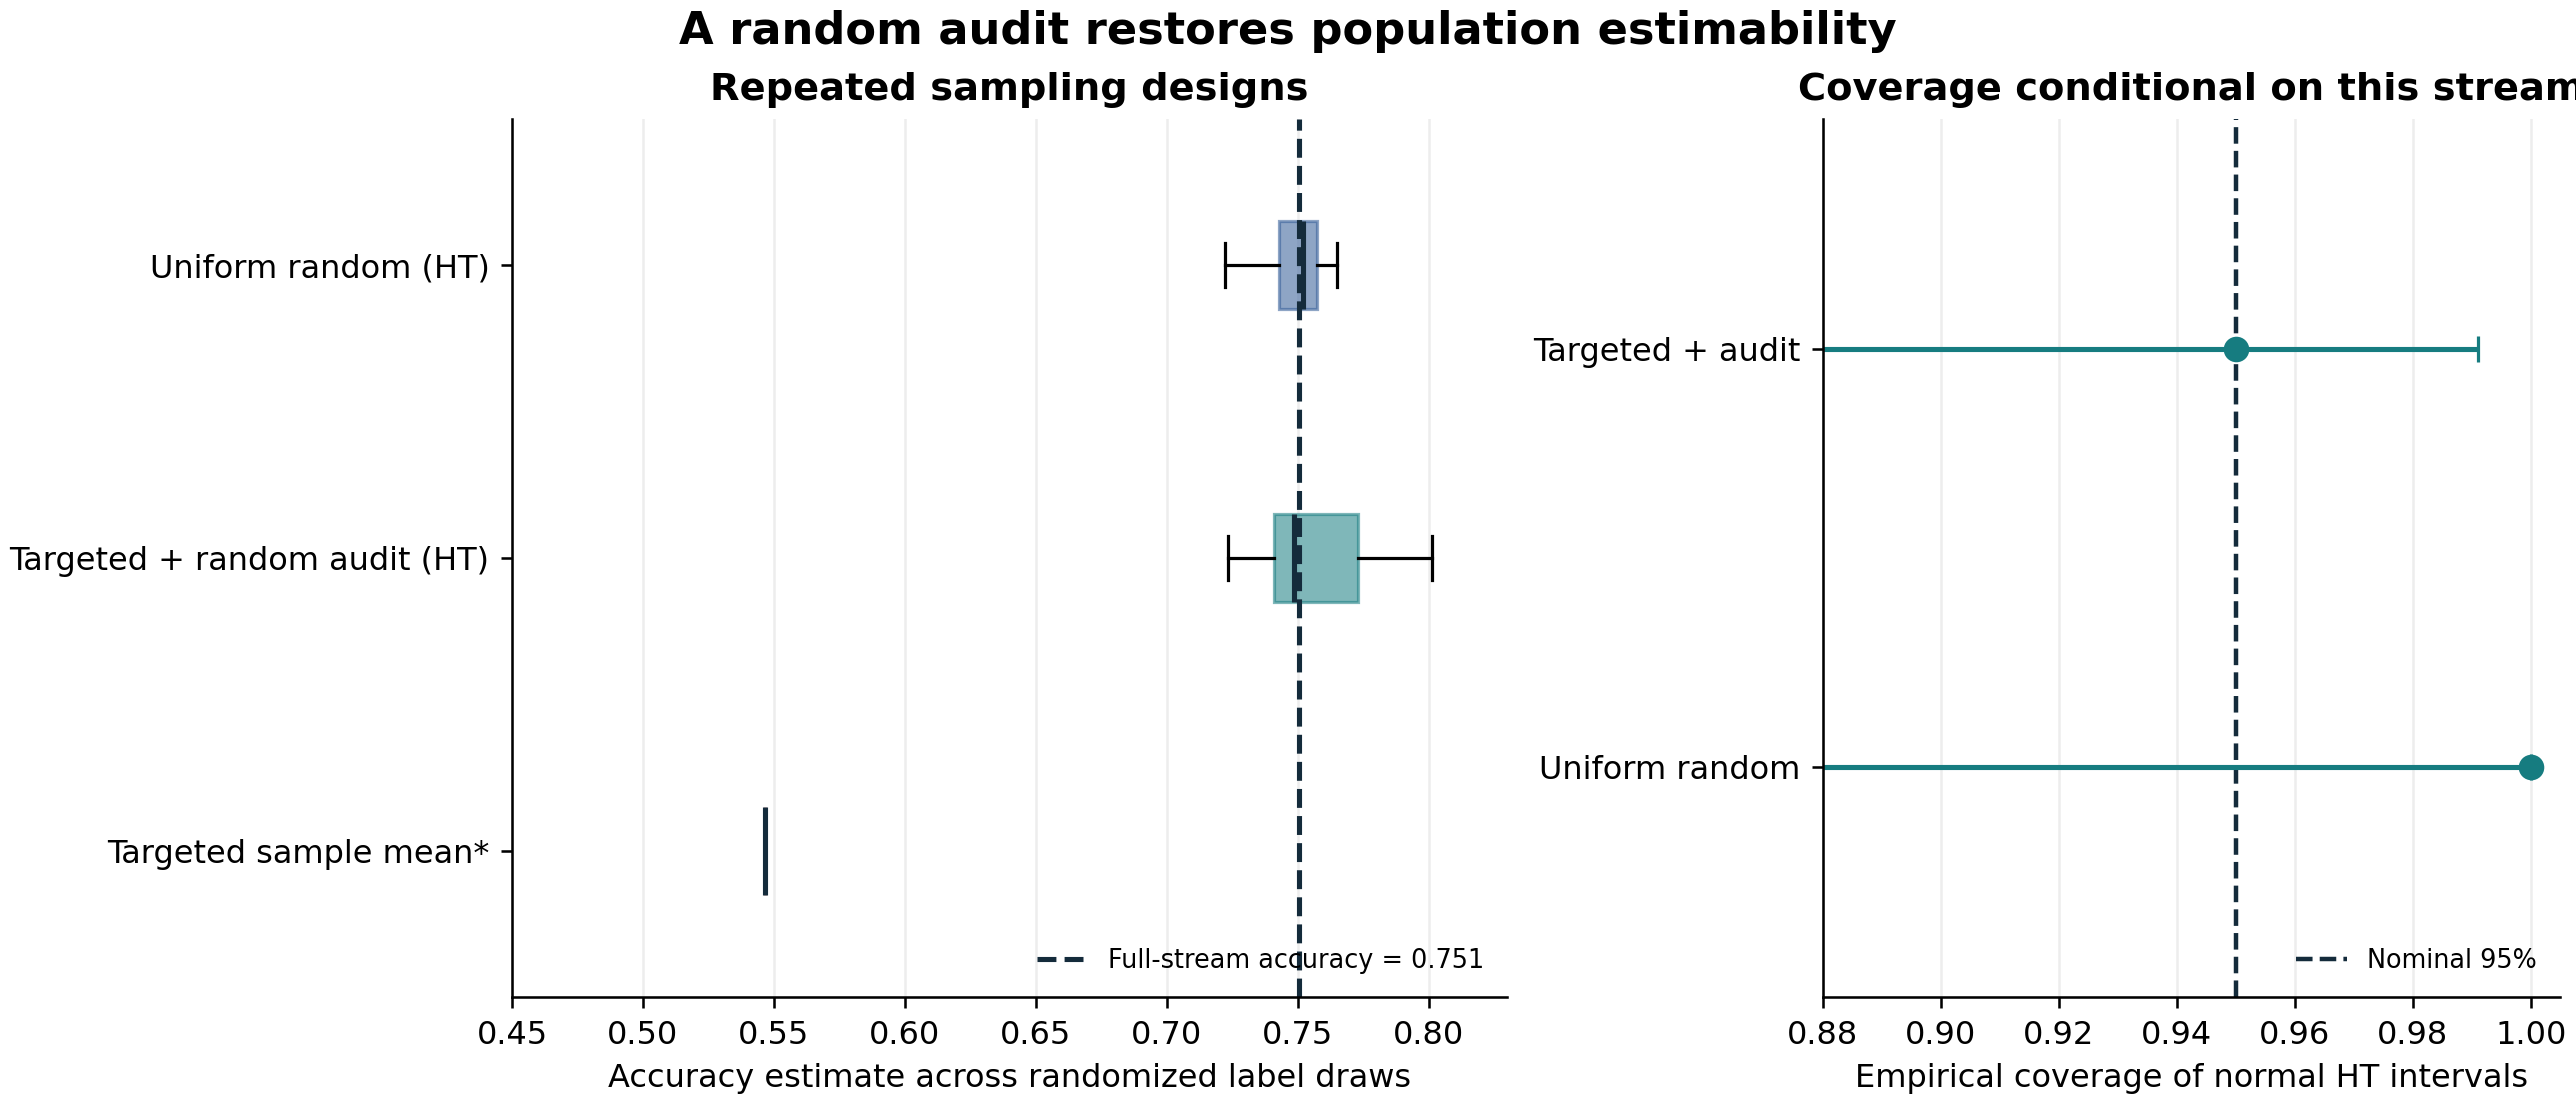
\includegraphics[width=\linewidth]{noaa_selective_design.png}\end{center}
\begin{table}[ht]\centering\small
\begin{tabular}{lrrrr}\toprule
Policy & Mean labels & Mean estimate & HT bias & 95\% interval coverage\\\midrule
Targeted only (naive descriptor) & 1050{} & 0.5467 & Not estimable & Not defined\\
Targeted + random audit (HT) & 2002.8{} & 0.7559 & +0.0053 & 95.0\%\\
Uniform random (HT) & 1997.5{} & 0.7518 & +0.0012 & 100.0\%\\\bottomrule
\end{tabular}
\caption{Averages across independent sampling draws on the one fixed NOAA stream. Coverage is conditional on that stream.}
\end{table}
\section*{Interpretation and limitations}
For this stream, the least-confident decile is much less accurate than the full population, so targeted-only labels substantially understate population accuracy. Adding a known-probability random audit makes the full-stream target design-estimable and gives near-nominal empirical coverage in this replay. The combined design's certainty stratum reduces effective sample size relative to uniform sampling despite similar label counts. This experiment does not establish prospective operations, repeated-domain uncertainty, nonresponse behavior, acquisition cost, selected-label recalibration, or validity under changing inclusion probabilities. The data are NOAA same-day completed summaries, and the task is retrospective classification.
\section*{Reproduction}
Run from the project root:
\begin{verbatim}
powershell -NoProfile -ExecutionPolicy Bypass \\
  -File .\scripts\reproduce_noaa_selective_label_replay.ps1 -Replicates 1000
\end{verbatim}
The audit receipt hashes sources, the locked NOAA evaluator, and every output. Row-level logs retain selected IDs, their inclusion probabilities, confidence-only acquisition score, prediction and selected correctness.
\end{document}
